\documentclass[]{article}
\usepackage{lmodern}
\usepackage{amssymb,amsmath}
\usepackage{ifxetex,ifluatex}
\usepackage{fixltx2e} % provides \textsubscript
\ifnum 0\ifxetex 1\fi\ifluatex 1\fi=0 % if pdftex
  \usepackage[T1]{fontenc}
  \usepackage[utf8]{inputenc}
\else % if luatex or xelatex
  \ifxetex
    \usepackage{mathspec}
  \else
    \usepackage{fontspec}
  \fi
  \defaultfontfeatures{Ligatures=TeX,Scale=MatchLowercase}
\fi
% use upquote if available, for straight quotes in verbatim environments
\IfFileExists{upquote.sty}{\usepackage{upquote}}{}
% use microtype if available
\IfFileExists{microtype.sty}{%
\usepackage{microtype}
\UseMicrotypeSet[protrusion]{basicmath} % disable protrusion for tt fonts
}{}
\usepackage[margin=1in]{geometry}
\usepackage{hyperref}
\hypersetup{unicode=true,
            pdftitle={ps7},
            pdfauthor={Ramon Crespo},
            pdfborder={0 0 0},
            breaklinks=true}
\urlstyle{same}  % don't use monospace font for urls
\usepackage{color}
\usepackage{fancyvrb}
\newcommand{\VerbBar}{|}
\newcommand{\VERB}{\Verb[commandchars=\\\{\}]}
\DefineVerbatimEnvironment{Highlighting}{Verbatim}{commandchars=\\\{\}}
% Add ',fontsize=\small' for more characters per line
\usepackage{framed}
\definecolor{shadecolor}{RGB}{248,248,248}
\newenvironment{Shaded}{\begin{snugshade}}{\end{snugshade}}
\newcommand{\AlertTok}[1]{\textcolor[rgb]{0.94,0.16,0.16}{#1}}
\newcommand{\AnnotationTok}[1]{\textcolor[rgb]{0.56,0.35,0.01}{\textbf{\textit{#1}}}}
\newcommand{\AttributeTok}[1]{\textcolor[rgb]{0.77,0.63,0.00}{#1}}
\newcommand{\BaseNTok}[1]{\textcolor[rgb]{0.00,0.00,0.81}{#1}}
\newcommand{\BuiltInTok}[1]{#1}
\newcommand{\CharTok}[1]{\textcolor[rgb]{0.31,0.60,0.02}{#1}}
\newcommand{\CommentTok}[1]{\textcolor[rgb]{0.56,0.35,0.01}{\textit{#1}}}
\newcommand{\CommentVarTok}[1]{\textcolor[rgb]{0.56,0.35,0.01}{\textbf{\textit{#1}}}}
\newcommand{\ConstantTok}[1]{\textcolor[rgb]{0.00,0.00,0.00}{#1}}
\newcommand{\ControlFlowTok}[1]{\textcolor[rgb]{0.13,0.29,0.53}{\textbf{#1}}}
\newcommand{\DataTypeTok}[1]{\textcolor[rgb]{0.13,0.29,0.53}{#1}}
\newcommand{\DecValTok}[1]{\textcolor[rgb]{0.00,0.00,0.81}{#1}}
\newcommand{\DocumentationTok}[1]{\textcolor[rgb]{0.56,0.35,0.01}{\textbf{\textit{#1}}}}
\newcommand{\ErrorTok}[1]{\textcolor[rgb]{0.64,0.00,0.00}{\textbf{#1}}}
\newcommand{\ExtensionTok}[1]{#1}
\newcommand{\FloatTok}[1]{\textcolor[rgb]{0.00,0.00,0.81}{#1}}
\newcommand{\FunctionTok}[1]{\textcolor[rgb]{0.00,0.00,0.00}{#1}}
\newcommand{\ImportTok}[1]{#1}
\newcommand{\InformationTok}[1]{\textcolor[rgb]{0.56,0.35,0.01}{\textbf{\textit{#1}}}}
\newcommand{\KeywordTok}[1]{\textcolor[rgb]{0.13,0.29,0.53}{\textbf{#1}}}
\newcommand{\NormalTok}[1]{#1}
\newcommand{\OperatorTok}[1]{\textcolor[rgb]{0.81,0.36,0.00}{\textbf{#1}}}
\newcommand{\OtherTok}[1]{\textcolor[rgb]{0.56,0.35,0.01}{#1}}
\newcommand{\PreprocessorTok}[1]{\textcolor[rgb]{0.56,0.35,0.01}{\textit{#1}}}
\newcommand{\RegionMarkerTok}[1]{#1}
\newcommand{\SpecialCharTok}[1]{\textcolor[rgb]{0.00,0.00,0.00}{#1}}
\newcommand{\SpecialStringTok}[1]{\textcolor[rgb]{0.31,0.60,0.02}{#1}}
\newcommand{\StringTok}[1]{\textcolor[rgb]{0.31,0.60,0.02}{#1}}
\newcommand{\VariableTok}[1]{\textcolor[rgb]{0.00,0.00,0.00}{#1}}
\newcommand{\VerbatimStringTok}[1]{\textcolor[rgb]{0.31,0.60,0.02}{#1}}
\newcommand{\WarningTok}[1]{\textcolor[rgb]{0.56,0.35,0.01}{\textbf{\textit{#1}}}}
\usepackage{graphicx,grffile}
\makeatletter
\def\maxwidth{\ifdim\Gin@nat@width>\linewidth\linewidth\else\Gin@nat@width\fi}
\def\maxheight{\ifdim\Gin@nat@height>\textheight\textheight\else\Gin@nat@height\fi}
\makeatother
% Scale images if necessary, so that they will not overflow the page
% margins by default, and it is still possible to overwrite the defaults
% using explicit options in \includegraphics[width, height, ...]{}
\setkeys{Gin}{width=\maxwidth,height=\maxheight,keepaspectratio}
\IfFileExists{parskip.sty}{%
\usepackage{parskip}
}{% else
\setlength{\parindent}{0pt}
\setlength{\parskip}{6pt plus 2pt minus 1pt}
}
\setlength{\emergencystretch}{3em}  % prevent overfull lines
\providecommand{\tightlist}{%
  \setlength{\itemsep}{0pt}\setlength{\parskip}{0pt}}
\setcounter{secnumdepth}{0}
% Redefines (sub)paragraphs to behave more like sections
\ifx\paragraph\undefined\else
\let\oldparagraph\paragraph
\renewcommand{\paragraph}[1]{\oldparagraph{#1}\mbox{}}
\fi
\ifx\subparagraph\undefined\else
\let\oldsubparagraph\subparagraph
\renewcommand{\subparagraph}[1]{\oldsubparagraph{#1}\mbox{}}
\fi

%%% Use protect on footnotes to avoid problems with footnotes in titles
\let\rmarkdownfootnote\footnote%
\def\footnote{\protect\rmarkdownfootnote}

%%% Change title format to be more compact
\usepackage{titling}

% Create subtitle command for use in maketitle
\newcommand{\subtitle}[1]{
  \posttitle{
    \begin{center}\large#1\end{center}
    }
}

\setlength{\droptitle}{-2em}

  \title{ps7}
    \pretitle{\vspace{\droptitle}\centering\huge}
  \posttitle{\par}
    \author{Ramon Crespo}
    \preauthor{\centering\large\emph}
  \postauthor{\par}
      \predate{\centering\large\emph}
  \postdate{\par}
    \date{11/15/2018}


\begin{document}
\maketitle

Notes: Worked on this problem by myself.

Problem 1 Suppose I have a statistical method that estimates a
regression coefficient and its standard error. I develop a simulation
study and have m = 1000 simulated datasets that each give me an estimate
of the coefficent and its standard error. How would I determine if the
statistical method properly characterizes the uncertainty of the
estimated regression coefficient?

A key element in determining the validity of the regression coeficients
is to check for bias results. In the context of linear regression, this
would be manifested in the linear regression model fitting a curve that
is center slightly of the expected mean.

\begin{Shaded}
\begin{Highlighting}[]
\NormalTok{devs <-}\StringTok{ }\KeywordTok{rnorm}\NormalTok{(}\DecValTok{100}\NormalTok{)}
\NormalTok{tdevs <-}\StringTok{ }\KeywordTok{qt}\NormalTok{(}\KeywordTok{pnorm}\NormalTok{(devs), }\DataTypeTok{df =} \DecValTok{1}\NormalTok{) }
\KeywordTok{plot}\NormalTok{(devs)}
\end{Highlighting}
\end{Shaded}

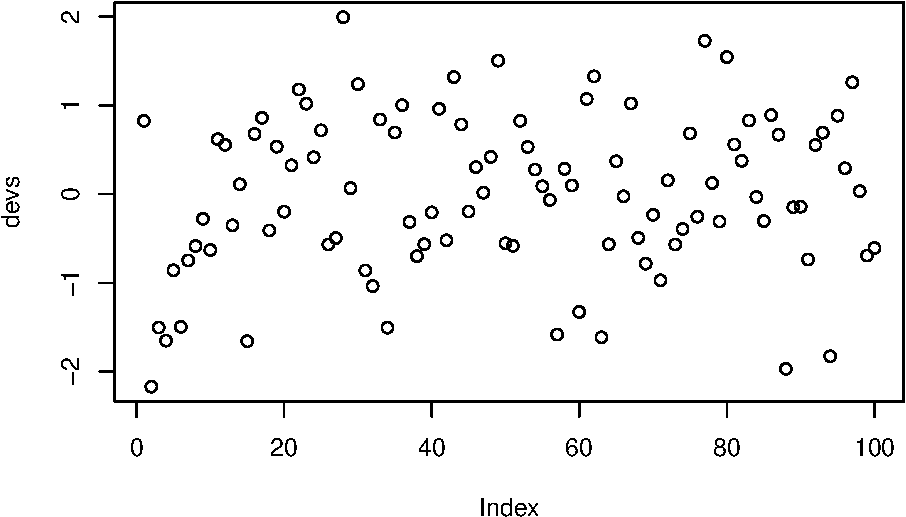
\includegraphics{ps7_files/figure-latex/unnamed-chunk-1-1.pdf}

Problem 2 Suppose I have a very large dataset, with n = 1e\^{}9, so I
have n observations and an n × p matrix X of predictors, where p = 8.
(a) Ordinarily, how much memory would the dataset take up? Complete
matrix = n = 1e9, d=8 --\textgreater{} 8e\^{}9 numbers * 8 bytes per
number = 64 GB

\begin{enumerate}
\def\labelenumi{(\alph{enumi})}
\setcounter{enumi}{1}
\item
  Now suppose that there are only 10000 unique combinations of the p
  covariates. Given what you know about data structures in R, how could
  you store the data to use up much less memory? How much memory would
  be used by your solution? You can store the 10000 unique combinations,
  10000\emph{8numbers}8bytes = 640,000 KB, and store an array of numbers
  that map the unique combinations to the values in the original matrix.
  The total space this takes is: 1e9\emph{1}8bytes + 640,000KB = 8.64GB
\item
  Now suppose you need to run lm(), glm(), etc. on this data. Why would
  all of your work in part (b) go to waste? The functions would have to
  build back the matrix to be able to compute the calculations. In other
  words the original matrix will need to be recomputed for the lm()
  function to fit the linear model.
\item
  If you need to find the OLS, (X.T\emph{X)\^{}-1}X.T\emph{Y estimator
  here, how could you code this up (please provide pseudo-code; you
  don't need to write any R code) so that you do not need to use up the
  full memory and can take advantage of your data structure(s). Problem
  statement: Performing calculations on datasets are specific to the
  structure and content of the dataset. For the purpose of this problem
  I will introduce some structure to the dataset so that my formulation
  makes sense. The context is the dataset consists of observations of
  the state of a system, and the entries in the dataset consist of how
  far the observations are from a reference state 0. You are mapping
  this observations to a rewar Y that is a function of the state d and
  some error e (Y is iid). The linear regression, would then be a
  predictor of rewards you can expect from visiting a specific state. In
  general, given that X = n x p matrix of and Y = p, it makes more sense
  to compute the operations in the following order =
  (X.T}X)\^{}-1\emph{(X.T}Y)
\end{enumerate}

Pseudo code -import matrix D and S where S is the matrix encoding the
10000 possible states and D is the map between S and the real data set R
-fit a model to the dataset D. -Step1: obtain E{[}Y{]},
E{[}(Y-E{[}Y{]})\^{}2{]} for each possible state by using the observed
rewards. This is computed using the reduced dataset containing the codes
for the states visited, not the actual states. -Step2: Now that you have
a distribution for the expected rewards in each state, you can sample
acual states and rewards by using the distributions. Sample from the
obtained distribution E{[}Y\textbar{}D{]}, E{[}(Y-E{[}Y{]})\^{}2{]} by
using rnorm(E{[}Y{]},E{[}(Y-E{[}Y{]})\^{}2). Choose a proper size for
the dataset, lets say 100000. -Step3: compute w =
(X.T\emph{X)\^{}-1}(X.T\emph{Y) by using the sampled dataset. -Step 3.1
= instead of solving the full problem above, use : QR decomposition. We
could try to use Cholesky decomposition but we depend on X.T}X being pd
which is highly unlikely because states are discrete thus some
repetition is highly likely): -QR Decomposition * X.T\emph{X}w =
X.T\emph{Y } R.T\emph{Q.T}.Q\emph{R}w = Q.T\emph{Y } R\emph{w = Q.T}Y
(this will be a backsolve since R is upper triangular)

-Step4: Check is results are consistent acros different simulations of
the above procedure, specially making sure that you have not created a
biased simulator that would lead to bias estimations of w.

The main point here is that in this context the actual data did not have
to be accessed, and distributions could be obtained by just using the
map (reduced dataset). Then expoit this structure to sample a smaller
dataset and fit a linear regression to the reduced dataset, that is
representative of the larger dataset.

\begin{enumerate}
\def\labelenumi{\arabic{enumi}.}
\setcounter{enumi}{2}
\tightlist
\item
  Suppose I need to compute the generalized least squares estimator, βˆ
  = (X.T\emph{Σ\^{}−1}X)\textsuperscript{−1\emph{X.T}Σ}−1*Y , for X n ×
  p, Σ n × n and assume that n \textgreater{} p.~Assume n could be of
  order several thousand and p of order in the hundreds. First write out
  in pseudo-code how you would do this in an efficient way - i.e., the
  particular linear algebra steps and the order of operations. Then
  write efficient R code in the form of a function, gls(), to do this -
  you can rely on the various high-level functions for matrix
  decompositions and solving systems of equations, but you should not
  use any code that already exists for doing generalized least squares.
\end{enumerate}

Basic Idea: 1) Separate the equation into efficient matrix and vector
operations 2) Avoid doing the naive inverse, solve a linear system of
equations instead 3) Avoid explicitly doing the transpose of matrices,
use code that computes that directly.

pseudo-code * compute the inverse of epsilon * a - compute the
crossproduct of X,epsilon * a - compute the crossproduct of a,X * a -
compute the inverse of a * b - compute the crossproduct of epsilon
inverse and Y * b - compute the crossproduct of X,b * c - compute the
crossproduct of a,b

\begin{Shaded}
\begin{Highlighting}[]
\NormalTok{n <-}\StringTok{ }\DecValTok{500}
\NormalTok{x <-}\StringTok{ }\KeywordTok{matrix}\NormalTok{(}\KeywordTok{rnorm}\NormalTok{(n}\OperatorTok{*}\NormalTok{n,}\DataTypeTok{mean=}\DecValTok{100}\NormalTok{,}\DataTypeTok{sd=}\DecValTok{2}\NormalTok{),}\DataTypeTok{nrow=}\NormalTok{n,}\DataTypeTok{ncol=}\NormalTok{n)}
\NormalTok{y <-}\StringTok{ }\KeywordTok{matrix}\NormalTok{(}\KeywordTok{rnorm}\NormalTok{(n,}\DataTypeTok{mean=}\DecValTok{80}\NormalTok{,}\DataTypeTok{sd=}\DecValTok{1}\NormalTok{),}\DataTypeTok{nrow=}\NormalTok{n,}\DataTypeTok{ncol=}\DecValTok{1}\NormalTok{)}
\NormalTok{gls <-}\StringTok{ }\ControlFlowTok{function}\NormalTok{(X,Y,epsilon) \{ }
\NormalTok{  eps_inv =}\StringTok{ }\KeywordTok{inv}\NormalTok{(epsilon)}
\NormalTok{  a =}\StringTok{ }\KeywordTok{inv}\NormalTok{(}\KeywordTok{crossprod}\NormalTok{(}\KeywordTok{tcrossprod}\NormalTok{(X,epsilon),X))}
\NormalTok{  b =}\StringTok{ }\KeywordTok{tcrosspro}\NormalTok{(X,}\KeywordTok{crossprod}\NormalTok{(eps_inv,Y))}
\NormalTok{  c =}\KeywordTok{crossprod}\NormalTok{(a,b)}
  \KeywordTok{return}\NormalTok{(c)}
\NormalTok{\}}
\end{Highlighting}
\end{Shaded}

\begin{enumerate}
\def\labelenumi{\arabic{enumi}.}
\setcounter{enumi}{3}
\tightlist
\item
  We've seen how to use Gaussian elimination (i.e., the LU
  decomposition) to solve Ax=b and that we can do the solution in
  n\^{}3/3 operations (plus lower-order terms). Now let's consider
  explicitly finding A−1 and then calculating x = A−1*b via
  matrix-vector multiplication. If we look at R's solve.default(), we
  see it solves the system AZ = I to find Z = A−1 and help(solve)
  indicates it calls a Lapack routine DGESV
  (\url{http://www.netlib.org/lapack/explore-html/d7/d3b/group__double_g_esolve_ga5ee879032a8365897c3ba91e}
  that uses the LU decomposition. Count the number of computations for
\end{enumerate}

\begin{enumerate}
\def\labelenumi{(\alph{enumi})}
\tightlist
\item
  transforming AZ = I to UZ = I∗ (where I∗ is no longer a diagonal
  matrix), This requires 2/3(n\^{}3). This corresponds to transforming
  matriz A into an upper triangular matrix
\item
  for solving for Z given UZ = I∗ O(n2)
\item
  for calculating x = Zb. O(n2)
\end{enumerate}

total complexity 2/3(n\^{}3)+2(n2)

\begin{enumerate}
\def\labelenumi{\arabic{enumi}.}
\setcounter{enumi}{4}
\tightlist
\item
  Compare the speed of b = X−1y using: (a) solve(X)\%*\%y, (b)
  solve(X,y), and (c) Cholesky decomposition followed by solving
  triangular systems. Do this for a matrix of size 5000 × 5000 using a
  single thread, using a matrix X constructed from W ⊤ W where the
  elements of the n × n matrix W are generated independently using
  rnorm().
\end{enumerate}

\begin{enumerate}
\def\labelenumi{(\alph{enumi})}
\tightlist
\item
  How do the timing and relative ordering amongst methods compare to the
  order of computations we discussed in class, the notes, and above in
  problem 4. The computational time are as follows:
\end{enumerate}

\begin{itemize}
\tightlist
\item
  solve(X)\%*\%y = 189s
\item
  solve(X,y) = 41s
\item
  Cholesky Decomposition = 26s
\end{itemize}

The cholesky decomposition is the fasted as expected. From class notes
an inclass work we know that LU O(n3) and Cholesky is also O(n3) but
involves only half as many calculations. This follows the results where
the Cholesky decomposition takes almost half of the time is takes
solve(X,y). The naive way is summarized in solve(X)\%*\%y where the
extra time and computational burdain comes from computing two separate
calculations, one is solving the system of linear equations and solving
for the identity matrix (solve(X)), and then using this solution times
the right hand side of the linear system to obtain the result of the
operations. From the previous questions we see that the computational
complexity of the naive method is quite higher that the computational
complexity of the more efficient methods, this follows the results in
this part of the problem

\begin{enumerate}
\def\labelenumi{(\alph{enumi})}
\setcounter{enumi}{1}
\tightlist
\item
  Are the results for b the same numerically for methods (b) and (c) (up
  to machine precision)? Comment on how many digits in the elements of b
  agree, and relate this to the condition number of the calculation.
\end{enumerate}

The results are not the same for b and c. As seen in the code below
there is a distance between the two solutions. This is a result of the
rounding error in the computation of the matrices. The from the
dataframe we conclude that the solutions are similar to the 5th decimal
point. The condition number in the matrices make the solutions
different, and specifically Cholesky decomposition is sensisitive to the
values in the matrix.

\begin{Shaded}
\begin{Highlighting}[]
\NormalTok{n <-}\StringTok{ }\DecValTok{5000}
\NormalTok{w <-}\StringTok{ }\KeywordTok{matrix}\NormalTok{(}\KeywordTok{rnorm}\NormalTok{(n}\OperatorTok{*}\NormalTok{n,}\DataTypeTok{mean=}\DecValTok{10}\NormalTok{,}\DataTypeTok{sd=}\DecValTok{2}\NormalTok{),}\DataTypeTok{nrow=}\NormalTok{n,}\DataTypeTok{ncol=}\NormalTok{n)}
\NormalTok{X <-}\StringTok{ }\KeywordTok{t}\NormalTok{(w) }\OperatorTok\StringTok{ }\NormalTok{w}
\NormalTok{y <-}\StringTok{ }\KeywordTok{matrix}\NormalTok{(}\KeywordTok{rnorm}\NormalTok{(n,}\DataTypeTok{mean=}\DecValTok{100}\NormalTok{,}\DataTypeTok{sd=}\DecValTok{10}\NormalTok{),}\DataTypeTok{nrow=}\NormalTok{n,}\DataTypeTok{ncol=}\DecValTok{1}\NormalTok{)}

\NormalTok{time_a <-}\KeywordTok{system.time}\NormalTok{(}
\NormalTok{a <-}\StringTok{ }\KeywordTok{solve}\NormalTok{(X)}\OperatorTok\NormalTok{y}
\NormalTok{)}

\NormalTok{time_b <-}\KeywordTok{system.time}\NormalTok{(}
\NormalTok{b <-}\StringTok{ }\KeywordTok{solve}\NormalTok{(X,y)}
\NormalTok{)}

\NormalTok{time_c_}\DecValTok{1}\NormalTok{ <-}\KeywordTok{system.time}\NormalTok{(}
\NormalTok{U <-}\StringTok{ }\KeywordTok{chol}\NormalTok{(X)}
\NormalTok{)}
\NormalTok{time_c_}\DecValTok{2}\NormalTok{ <-}\KeywordTok{system.time}\NormalTok{(}
\NormalTok{c_ <-}\StringTok{ }\KeywordTok{backsolve}\NormalTok{(U, }\KeywordTok{backsolve}\NormalTok{(U, y, }\DataTypeTok{transpose =} \OtherTok{TRUE}\NormalTok{))}
\NormalTok{)}
\KeywordTok{print}\NormalTok{(time_a)}
\end{Highlighting}
\end{Shaded}

\begin{verbatim}
##    user  system elapsed 
## 172.536   3.470 191.345
\end{verbatim}

\begin{Shaded}
\begin{Highlighting}[]
\KeywordTok{print}\NormalTok{(time_b)}
\end{Highlighting}
\end{Shaded}

\begin{verbatim}
##    user  system elapsed 
##  35.039   0.256  35.581
\end{verbatim}

\begin{Shaded}
\begin{Highlighting}[]
\KeywordTok{print}\NormalTok{(time_c_}\DecValTok{1}\NormalTok{)}
\end{Highlighting}
\end{Shaded}

\begin{verbatim}
##    user  system elapsed 
##  23.903   0.165  24.235
\end{verbatim}

\begin{Shaded}
\begin{Highlighting}[]
\KeywordTok{print}\NormalTok{(time_c_}\DecValTok{2}\NormalTok{)}
\end{Highlighting}
\end{Shaded}

\begin{verbatim}
##    user  system elapsed 
##   0.030   0.001   0.030
\end{verbatim}

\begin{Shaded}
\begin{Highlighting}[]
\NormalTok{df <-}\StringTok{ }\KeywordTok{data.frame}\NormalTok{(b,c_)}
\NormalTok{df[}\DecValTok{0}\OperatorTok{:}\DecValTok{10}\NormalTok{,]}
\end{Highlighting}
\end{Shaded}

\begin{verbatim}
##              b          c_
## 1   3964.95487  3964.99192
## 2   3601.96797  3602.04142
## 3   4328.08279  4328.13869
## 4   1145.60897  1145.62522
## 5   1273.26839  1273.30334
## 6    -43.24143   -43.25153
## 7   1199.78864  1199.79397
## 8   3586.83451  3586.86939
## 9   -290.94888  -290.92079
## 10 -3642.88362 -3642.92315
\end{verbatim}


\end{document}
